\chapter{Methods}
\label{chp:methods}


%% Vi kan sikkert skrive litt om dette i metode

% \subsection{Version Control}
% \label{subsec:version-control}

% The use of \gls{git} as a version control system enables collaborative development by allowing multiple developers to work on the same codebase simultaneously. \gls{git} facilitates the maintenance of the code and provides a comprehensive history of all modifications made to the project. These changes are tracked within project containers known as \glspl{repository}, ensuring transparency and accountability throughout the development process. \cite{alphaefficiency:git}

% \subsubsection*{Branches}

% Git utilizes branches, which are independent lines of development within a repository. Branches allow developers to work on new features, fixes, or experiments without affecting the main codebase. Once changes in a branch are tested and finalized, they can be merged back into the main branch, ensuring a streamlined and controlled integration process. Branching supports parallel development and helps prevent conflicts by isolating work until it's ready for review and integration. \cite{git:branches}

\begin{center}
    \textit{Here, the development process and methodologies are described in detail. This includes the design and implementation of the desktop application, the selection of tools and frameworks, and the approach to solving the problem.}
\end{center}



\section{Machine Learning Models}
\label{sec:ml-models}

After conducting research into existing chess digitization methods, a publicly available solution developed by Peter Batchelor, Tom Richardson, and other contributors was identified. This solution serves as the foundation for our approach. It utilizes two \glspl{cnn}: one for detecting chess pieces and another for locating the squares of the chessboard \cite{lichess:chesscam}. \\

Although the documentation for the models was limited, the necessary logic and structure of the models were already present in the repository itself. When additional clarifications were needed, they were obtained through direct communication with the original developers, ensuring that the intended use and functionality of the models were correctly understood. 

\subsection*{Format Selection and Preprocessing}
The ChessCam repository provided multiple model formats, including PyTorch and ONNX. The ONNX format was chosen because it is framework-agnostic, making integration into different deployment environments easier. Before the models could be used, several preparatory steps were required. Netron was employed to inspect the ONNX files and determine the expected input and output. \\

\newpage


\subsection{Piece Detection Model}
\subsubsection*{Inputs and outputs}
The piece detection model is responsible for identifying and classifying chess pieces on the board. It expects input in the format \textbf{[1, 3, 288, 480]}. \textbf{1} represents the batch size, i.e., the number of images processed at once, which is typically set to 1 during inference. \textbf{3} corresponds to the number of color channels (RGB), indicating that the image must be in color. \textbf{288} and \textbf{480} denote the height and width of the image in pixels, respectively. \\

The model outputs data in the format \textbf{[1, 16, 2835]}. \textbf{1} represents the batch size, consistent with the input format. \textbf{16} consists of two parts: \begin{itemize} \item The first 4 values correspond to the bounding box coordinates for each predicted piece. These are not the final bounding box coordinates but rather the adjustments (offsets) relative to predefined anchor boxes within the image. \item The remaining 12 values represent the class probabilities for each possible piece type (e.g., black pawn, white knight, etc.). With 12 possible classes for the chess pieces, the model outputs 12 probabilities for each anchor box. \end{itemize} \\

\begin{table}[ht]
\centering
\caption{Chess Piece Classification Labels}
\begin{tabular}{|c|c|}
\hline
\multicolumn{2}{|c|}{\textbf{Model Labels}} \\  % Adds a row at the top
\hline
\textbf{Black Pawn} & \textbf{White Pawn} \\
\textbf{Black Knight} & \textbf{White Knight} \\
\textbf{Black Bishop} & \textbf{White Bishop} \\
\textbf{Black Rook} & \textbf{White Rook} \\
\textbf{Black Queen} & \textbf{White Queen} \\
\textbf{Black King} & \textbf{White King} \\
\hline
\end{tabular}
\end{table}


\textbf{2835} represents the number of anchor boxes used in the detection. These are predefined bounding boxes of various sizes and aspect ratios distributed across the image and act as potential locations for chess pieces. \\

To summarize: there are 2835 predefined anchor boxes spread across the image, each serving as a candidate location for detecting a chess piece. During training, the model learns to adjust these anchor boxes to better match the actual pieces on the board. It achieves this by predicting 4 offset values that modify the location and size of each anchor box. At runtime, for each anchor box, the model uses these learned offsets and outputs 12 class probabilities, indicating the likelihood of each chess piece type being present at that location. An example is illustrated in Table~\ref{tab:anchor-box-table}).

\newpage

\begin{table}[h]
    \centering
    \caption{Probabilities for each label for each anchor box}  % Caption moved to top
    \renewcommand{\arraystretch}{1.5} % Increase row height to allow text to be on top
    \begin{tabular}{lcccc}
        \toprule
        \textbf{Anchor box} & \textbf{Black Pawn} & \textbf{White Pawn} & \textbf{Black Knight} & \textbf{...} \\
        \midrule
        Anchor box 1 & \raggedright 0.03 & \raggedright 0.71 & \raggedright 0.01 & ... \\
        Anchor box 2 & \raggedright 0.82 & \raggedright 0.02 & \raggedright 0.01 & ... \\
        Anchor box 3 & \raggedright 0.02 & \raggedright 0.01 & \raggedright 0.78 & ... \\
        ... & ... & ... & ... & ... \\
        Anchor box 2835 & \raggedright 0.01 & \raggedright 0.03 & \raggedright 0.05 & ... \\
        \bottomrule
    \end{tabular}
    \label{tab:anchor-box-table}
\end{table}



\subsubsection*{Implementation}

he piece detection model is responsible for identifying and classifying chess pieces. It expects an input image of size 288x480 with three color channels. Since video frames typically do not come in this exact format, the images are first scaled to the required dimensions to ensure compatibility with the model.

There are in total 12 class labels each for the type piece and which color it is.

After processing the image, the model returns a set of predictions for each potential piece. These predictions include:

The model predicts these values for each anchor box. An anchor box is a predefined bounding box within the image that serves as a potential candidate location for a piece. By adjusting these anchor boxes, the model can detect and classify pieces across different positions on the chessboard.


\begin{subfigure}[h!]{0.9\linewidth} \centering 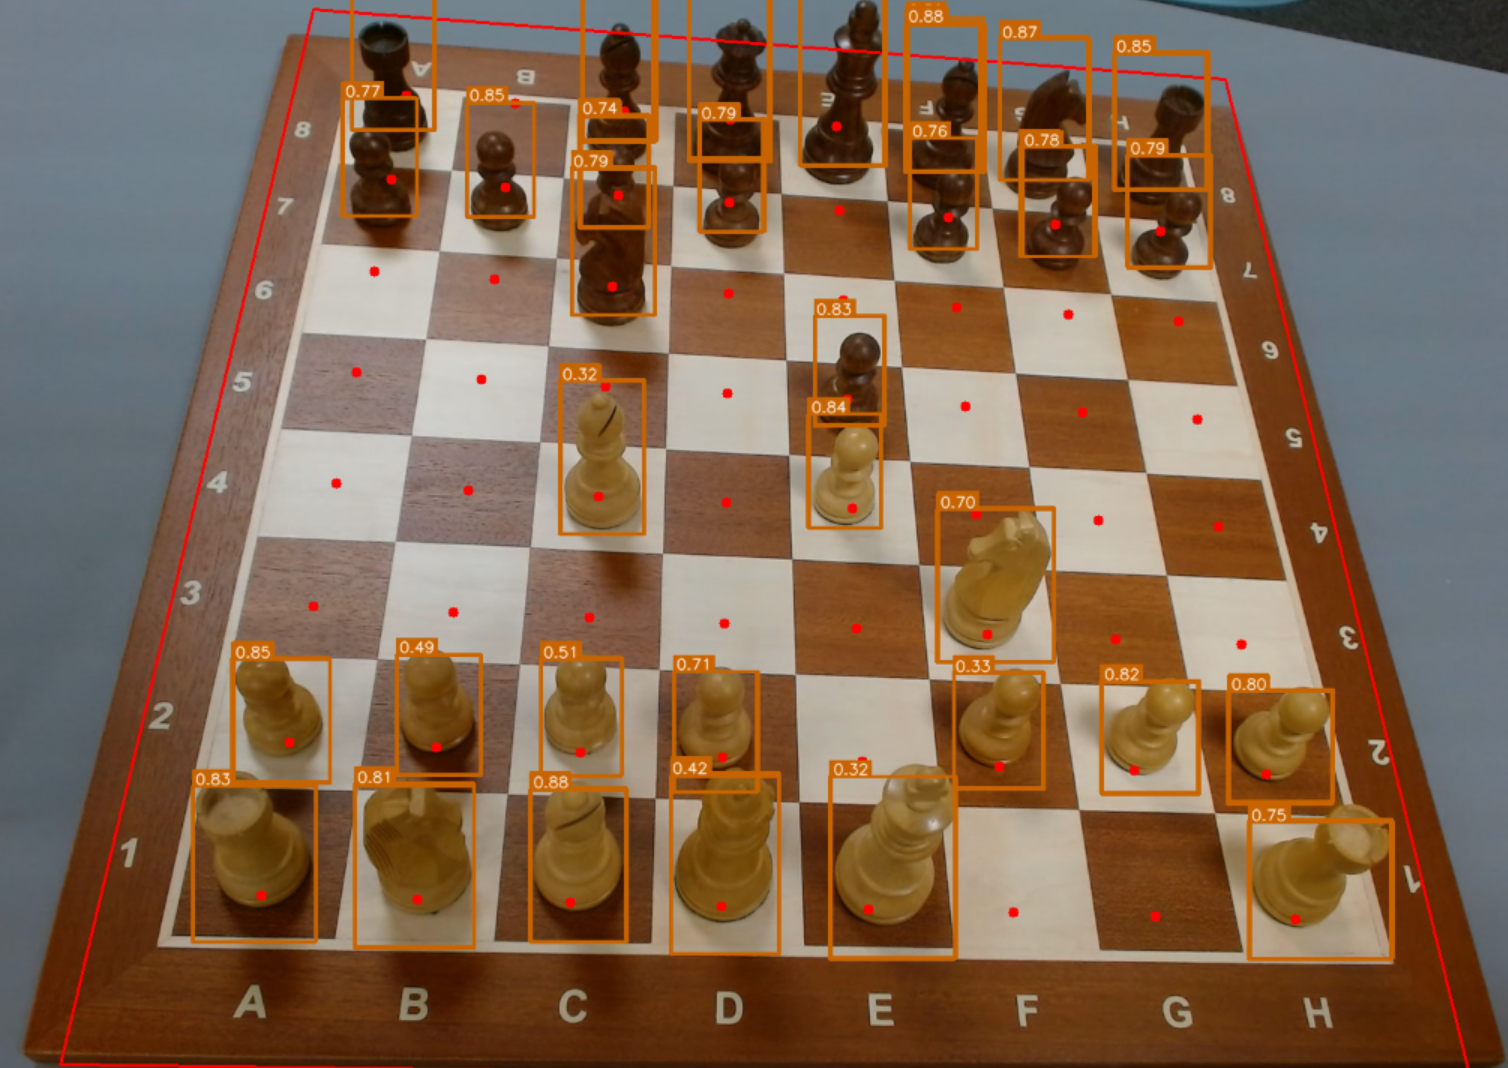
\includegraphics[width=\linewidth]{figures/methods/ml-models/piece-model.png} \caption{Tournament View} \end{subfigure}



\section{Development Methodology}
\label{sec:development-methodology}

\subsection{Agile Approach}
\label{subsec:agile-approach}

During the development of the application, Agile software development methodologies were adopted. This approach was chosen to support flexibility, collaboration, and customer satisfaction throughout the project lifecycle.

\subsubsection*{Sprints}

The team conducted bi-weekly meeting, each concluded with a sprint review and retrospective. Sprint planning involved discussions around:

\begin{itemize}
  \item \textbf{Sprint Goals:} Individual objectives and tasks to be completed before the next meeting.
  \item \textbf{Completed Tasks:} A review of which issues were resolved during the sprint.
  \item \textbf{Incomplete Tasks:} Identification of tasks that were not successfully completed and possible causes.
  \item \textbf{Next Sprint Planning:} General objectives for the upcoming sprint.
  \item \textbf{Action Items:} Assignments clarifying who would be responsible for specific tasks.
  \item \textbf{Product Backlog Review:} Selection of tasks to work on during the next sprint.
\end{itemize}

During retrospectives, the team reflected on what went well during the sprint and identified areas for improvement, fostering continuous learning and adaptation.

\subsubsection*{Product Owner}

\subsubsection*{Supervisor}

\subsubsection*{Issue Board}

To manage and track tasks, the team utilized GitHub’s Issue Board. Each issue was categorized based on its type:
\begin{itemize}
  \item \textbf{Feature/Enhancement:} New functionality or improvements.
  \item \textbf{Documentation:} Work related to improving documentation and team understanding.
  \item \textbf{Bug:} Issues related to errors or unexpected behavior in the application.
  \item \textbf{Task:} General tasks not fitting into the other categories.
\end{itemize}

Each issue was assigned to one or more team members to clarify responsibilities. The Issue Board was divided into four columns:
\textit{No Status}, \textit{To Do}, \textit{In Progress}, and \textit{Done}, offering a clear visual overview of the development workflow.

\subsubsection*{Code Review}

In alignment with the workflow described in Subsection~\ref{subsec:version-control}, as outlined in Chapter \ref{chp:theory}, each issue was implemented on a dedicated branch. This setup enabled team members to conduct peer reviews via GitHub pull requests before merging changes into the main codebase. This process encouraged collaboration, maintained code quality, and facilitated shared decision-making within the team.

\newpage

\section{Software Design}
\label{sec:software-design}

Regarding the design of the product, the product owner expressed no particular preferences and allowed the team full control in determining the website’s structure and color palette.

\subsection{Design Process}
\label{subsec:design-process}

The following processes align with the principles discussed in \ref{subsubsec:usability-testing}, as outlined in Chapter~\ref{chp:theory}.

\subsubsection*{User-Centered Design}
\label{subsubsec:user-centered-design}

At the beginning of the design process, the group conducted wireframe testing with a diverse set of users. This included participants of varying age groups—from young to elderly—as well as both chess players and non-chess players. The goal was to evaluate whether users found the interface intuitive and whether the sizing and layout were appropriate across different demographics. \\

All participants were given the same context before starting the test: 

\begin{quote}
\textit{You are viewing a chess game between two companions you know. You visit the tournament organizer's website and come across this webpage.}
\end{quote}

Participants were then either given specific tasks to perform within the application or asked to explore freely, mimicking a real-world scenario. This approach aimed to identify how naturally users could navigate and understand the application without explicit instruction. \\

After completing their interaction with the application, participants filled out an anonymous feedback form. This encouraged honest, unfiltered responses, reducing the likelihood of social desirability bias. The form included questions such as:

\begin{itemize}
    \item \textit{On a scale from 1 to 5, how satisfied are you with the overall experience of the application?}
    \item \textit{On a scale from 1 to 5, how satisfied are you with the Tournament View page?}
    \item \textit{On a scale from 1 to 5, how satisfied are you with the Board View page?}
    \item \textit{Do you have any feedback, suggestions for improvement, or features you would like to see added?}
\end{itemize}

See Subsection \ref{subsec:wireframe} for the final tested wireframe.

\newpage

\subsubsection*{Color Palette}
\label{subsubsec:color-palette}

In selecting the application's color palette, the group opted for a variation of blue. This choice was influenced by the symbolic associations of the color blue, which is often linked to imagination, intelligence, and wisdom \cite{blue}—qualities that align closely with the nature of chess \cite{chess:ppqty, chess:chess-and-creativity}. \\

To identify the most suitable stylistic direction, several versions of the application were developed, each showcasing a distinct color palette. These prototypes were printed and displayed in a shared space, allowing individuals from diverse backgrounds to view and compare them. \\

Participants were invited to vote for their preferred versions via a form. Each participant was allowed up to three votes and had the option to leave comments. For instance, some expressed a preference for the light mode from palette \#08 and the dark mode from palette \#07, while others favored the board design from palette \#05 or the move-highlighting style from palette \#14. \\

Rather than selecting a single predefined palette, the final color scheme was assembled by combining the most highly rated elements across the top-voted variations. This approach allowed for a more tailored and user-informed visual design (See Figure \ref{fig:color-palette-results} for the vote results). \\

\begin{figure}[h!]
    \centering
    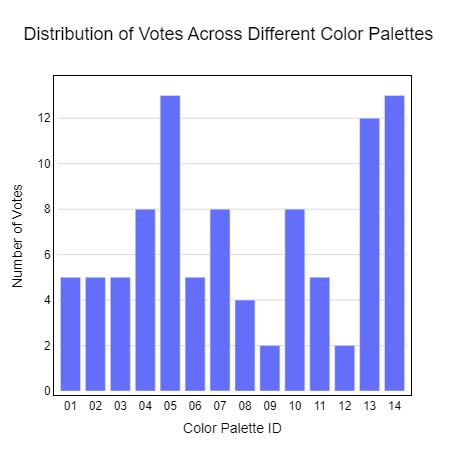
\includegraphics[width=0.75\linewidth]{figures/methods/color-palette-results.png}
    \caption{Distribution of Votes Across Different Color Palettes}
    \label{fig:color-palette-results}
\end{figure}

See Appendix~\ref{app:color-palettes} for the full set of tested color palettes.

\subsection{Diagrams}
\label{subsec:diagrams}

To provide a comprehensive understanding of the system architecture and interaction flow, several \gls{uml} diagrams were created. These diagrams model different aspects of the live chess game digitization system, from component interactions and activity flow to user roles and use cases.

\subsubsection*{Sequence Diagram}
\label{subsubsec:sequence-diagram}

The sequence diagram, shown in Figure \ref{fig:sequence}, illustrates the chronological flow of interactions between the system components and external actors. It begins with the Admin initiating the game recording by setting up the camera, which captures and streams the board state to a local processing unit. This unit continuously detects and validates moves, updating the user interface accordingly. Users, from remote devices, can spectate the game in real time or save it as a \gls{pgn} file. The diagram emphasizes the communication between hardware (camera and local machine) and the \gls{ui}, highlighting how physical chess games are digitized and broadcasted.

\begin{figure}[h!]
    \centering
    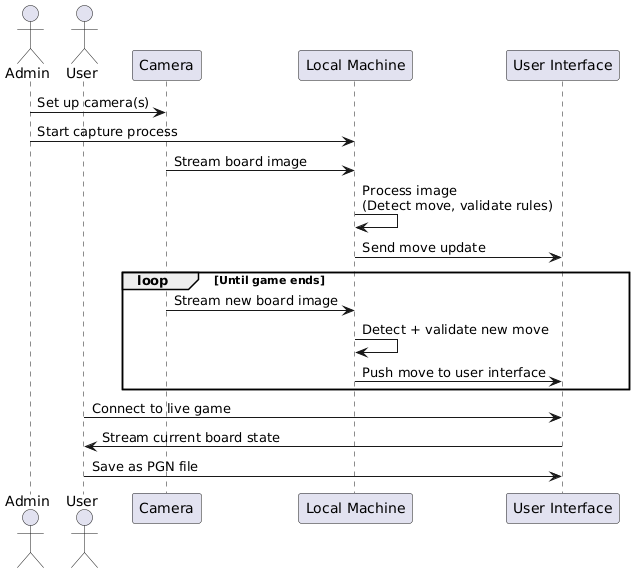
\includegraphics[width=0.75\linewidth]{figures/methods/uml/sequence.png}
    \caption[Sequence Diagram]{Sequence Diagram}
    \label{fig:sequence}
\end{figure}

\subsubsection*{Use-Case Diagram}
\label{subsubsec:use-case-diagram}

The use-case diagram, shown in Figure \ref{fig:use-case}, identifies the system’s main actors and the primary functionalities they interact with. Admins are responsible for hardware setup and initiating the game recording process. The system autonomously handles move detection, validation, and \gls{ui} updates. Users, on the other hand, access the game remotely to spectate or download \gls{pgn} files. This diagram provides a clear overview of who interacts with the system and what capabilities are exposed, forming the basis for understanding system requirements and user expectations.

\begin{figure}[h!]
    \centering
    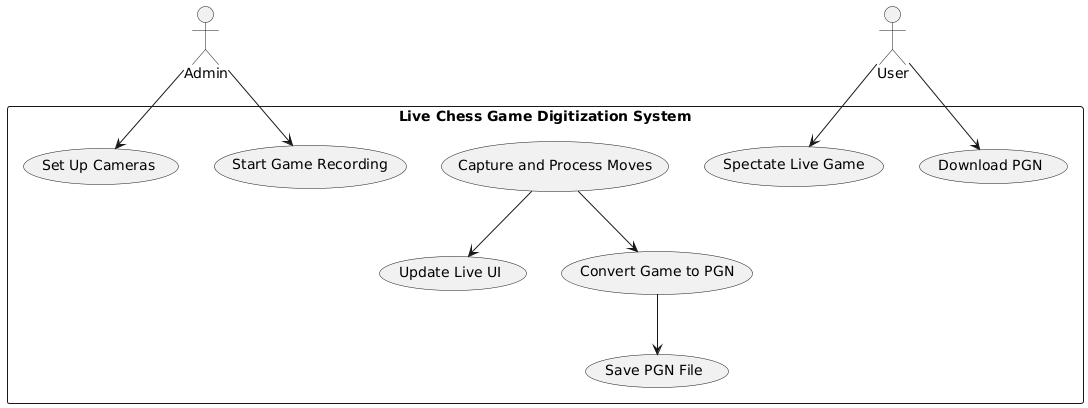
\includegraphics[width=0.75\linewidth]{figures/methods/uml/use-case.png}
    \caption{Use-Case Diagram}
    \label{fig:use-case}
\end{figure}

\begin{figure}[h!]
    \subsubsection*{Activity Diagram}
    \label{subsubsec:activity-diagram}
    
    \centering
    \begin{minipage}[t]{0.5\textwidth}
        \vspace{0pt}
        The activity diagram, shown in Figure \ref{fig:activity}, provides a high-level overview of the operational workflow during a chess game session. It models the continuous loop of capturing board states, detecting and validating moves, and updating the game state until the game ends. If a move is invalid, the system flags it but does not terminate the session. Once the game concludes, it is converted into a standard \gls{pgn} format. This diagram emphasizes the logical flow and decision-making process, reflecting the system’s role in automating and maintaining the integrity of live digitization.
    \end{minipage}
    \hfill
    \begin{minipage}[t]{0.45\textwidth}
        \vspace{0pt}
        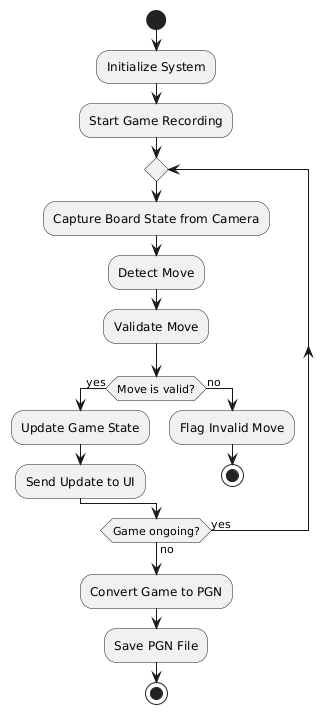
\includegraphics[width=\linewidth]{figures/methods/uml/activity-2.png}
        \caption[Activity Diagram]{Activity Diagram}
        \label{fig:activity}
    \end{minipage}
\end{figure}

\subsection{Wireframes}
\label{subsec:wireframe}

\subsubsection*{Control Panel}

The Control Panel, Figure \ref{fig:control-panel-group}, is a desktop-only interface designed for tournament organizers to manage the digitization of multiple physical chess boards. The interface follows a simple three-step workflow:

\begin{enumerate}
    \item \textbf{Select Number of Cameras:} The admin specifies how many boards will be monitored, which informs the system how many camera feeds to initialize, Figure \ref{fig:control-panel-1}.
    \item \textbf{Start Cameras and Digitization:} This action triggers the camera feeds, board state recognition, and move validation processes, Figure \ref{fig:control-panel-2}.
    \item \textbf{Restart Boards for New Round:} At the end of a round, this step resets the system state across all boards, preparing it for the next set of games, Figure \ref{fig:control-panel-3}.
\end{enumerate}

The control panel is intentionally minimal and task-oriented, ensuring admins can quickly configure and manage the system with minimal technical overhead.

\begin{figure}[h!]
    \centering
    \begin{subfigure}[h!]{0.45\linewidth}
        \centering
        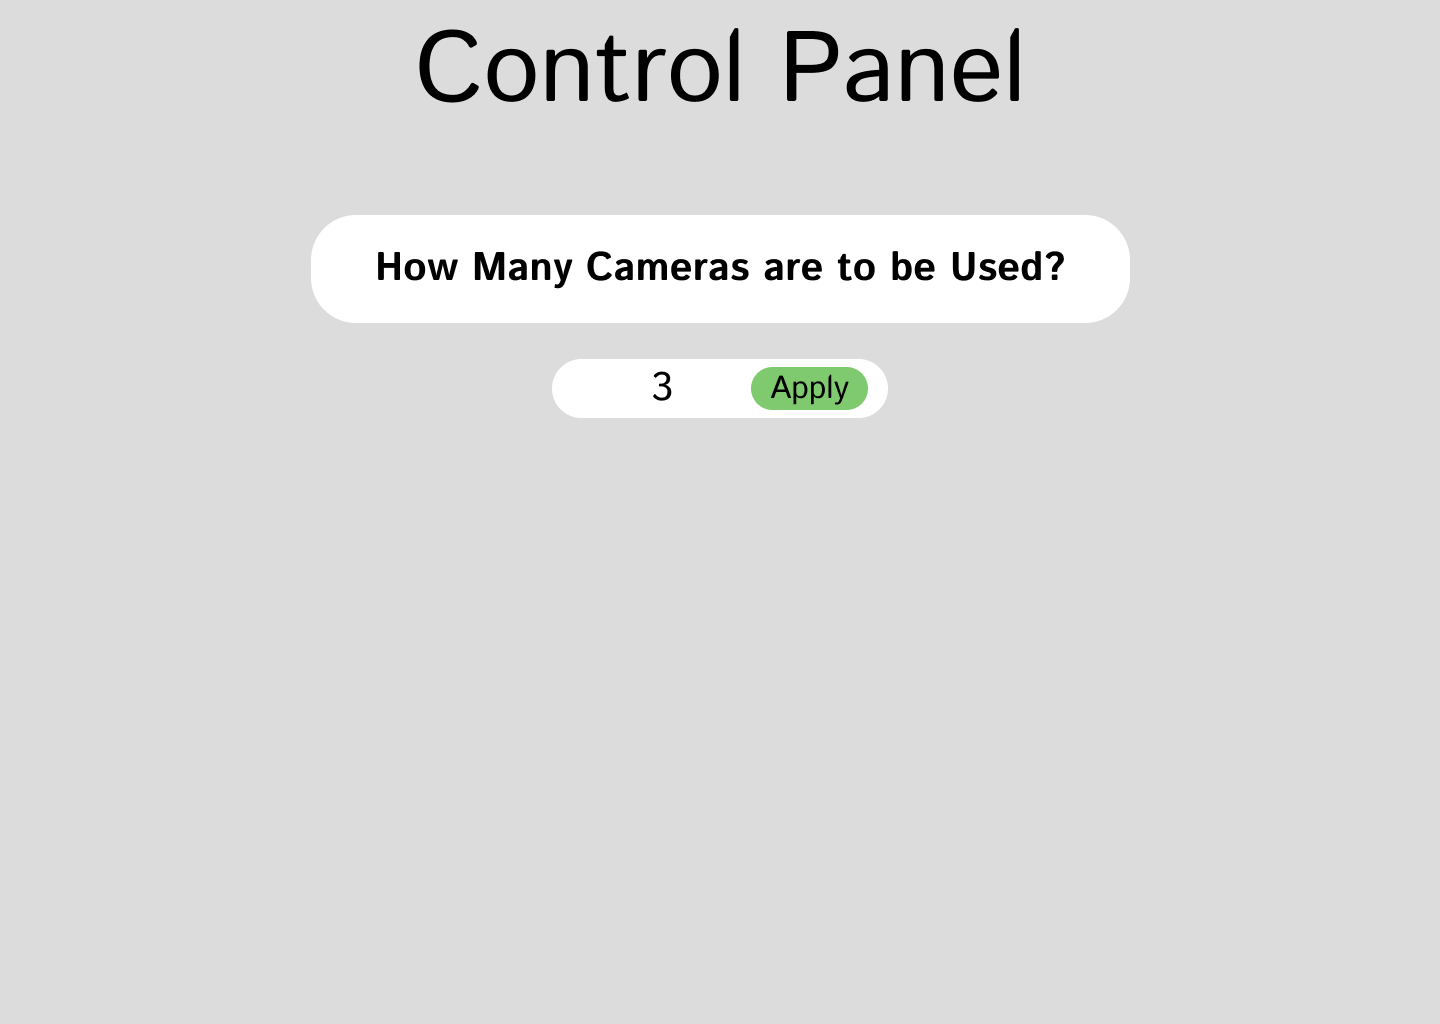
\includegraphics[width=\linewidth]{figures/methods/wireframes/control-panel-1.png}
        \caption{Step 1}
        \label{fig:control-panel-1}
    \end{subfigure}
    \hfill
    \begin{subfigure}[h!]{0.45\linewidth}
        \centering
        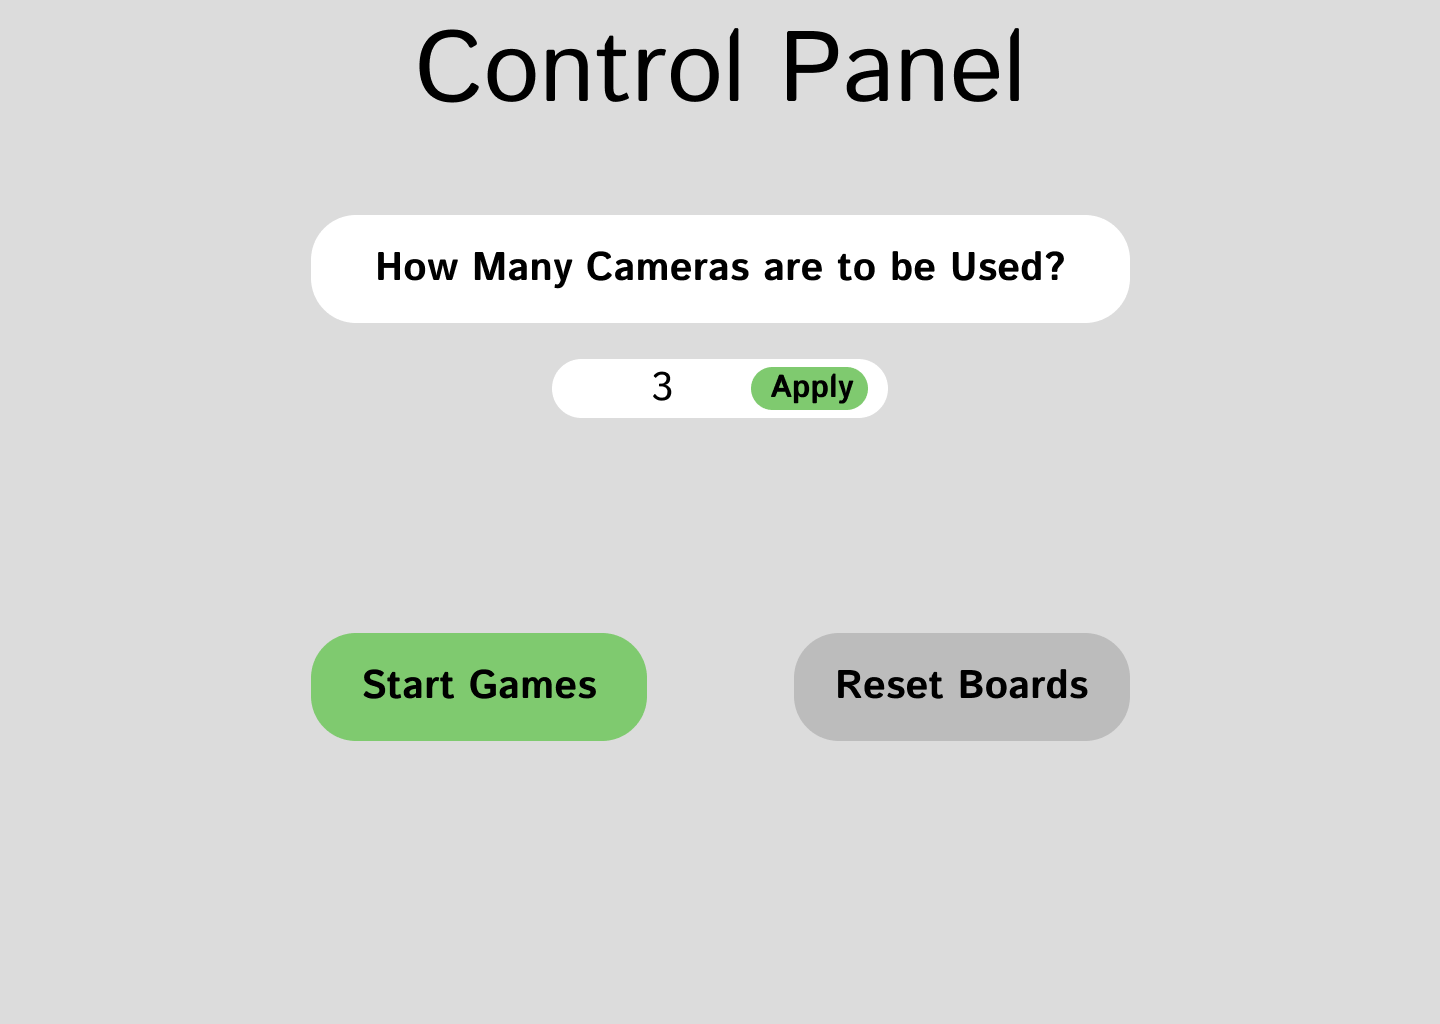
\includegraphics[width=\linewidth]{figures/methods/wireframes/control-panel-2.png}
        \caption{Step 2}
        \label{fig:control-panel-2}
    \end{subfigure}
    
    \vspace{1em}

    \begin{subfigure}[h!]{0.45\linewidth}
        \centering
        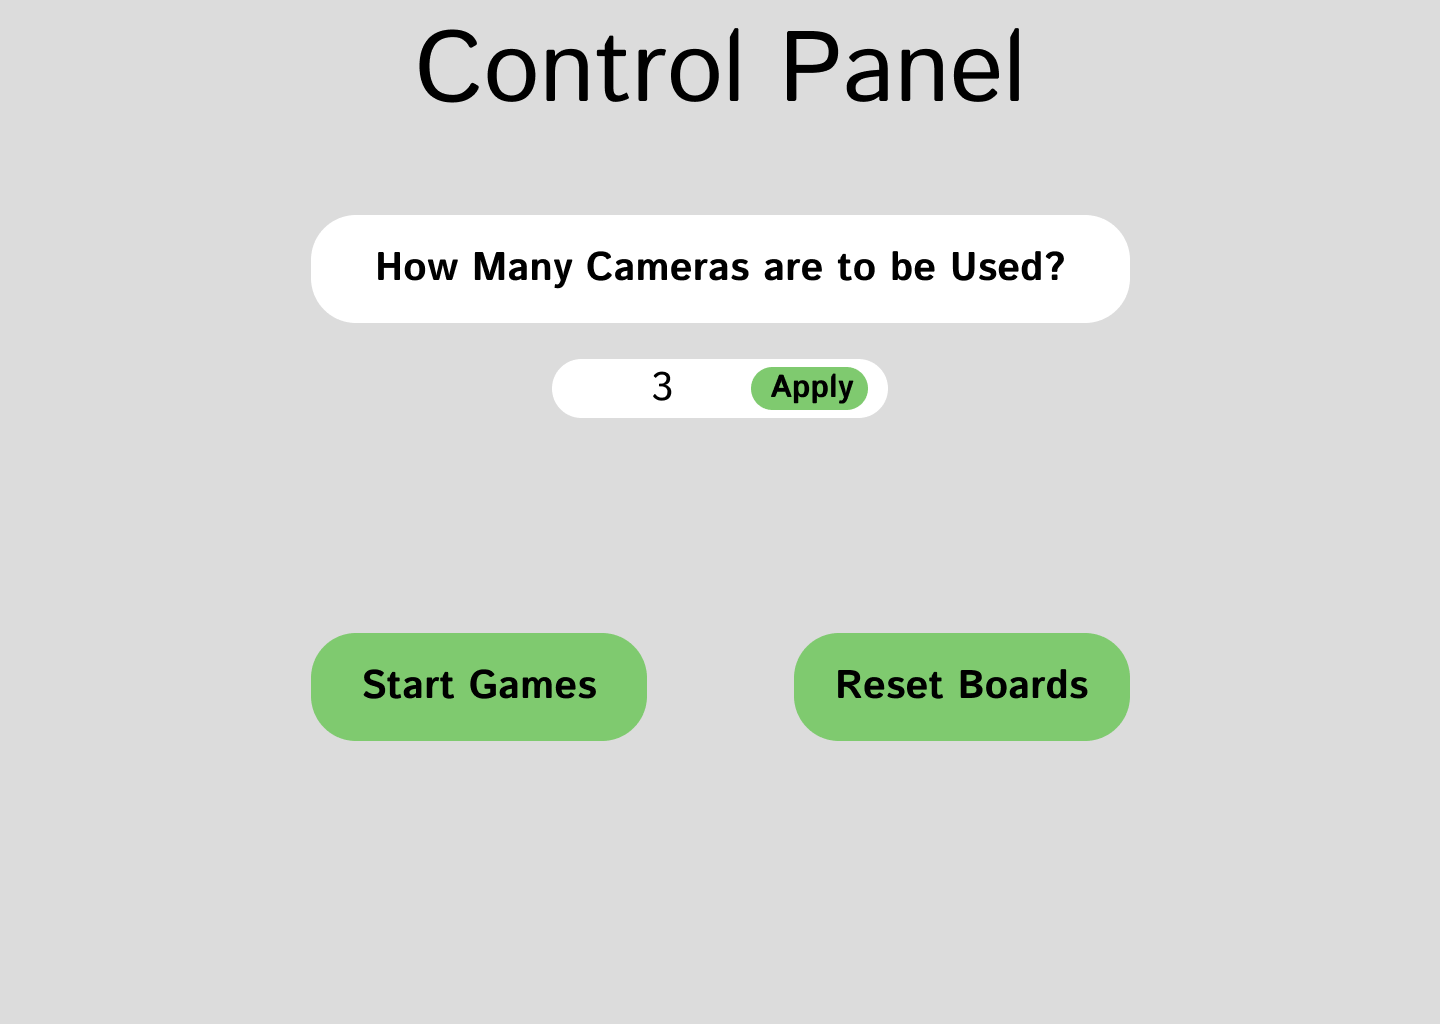
\includegraphics[width=\linewidth]{figures/methods/wireframes/control-panel-3.png}
        \caption{Step 3}
        \label{fig:control-panel-3}
    \end{subfigure}
    
    \caption{Control Panel wireframes showing sequential interaction steps}
    \label{fig:control-panel-group}
\end{figure}

\begin{figure}[h!]
\subsubsection*{Desktop View}
    \centering
    \begin{subfigure}[h!]{0.45\linewidth}
        \centering
        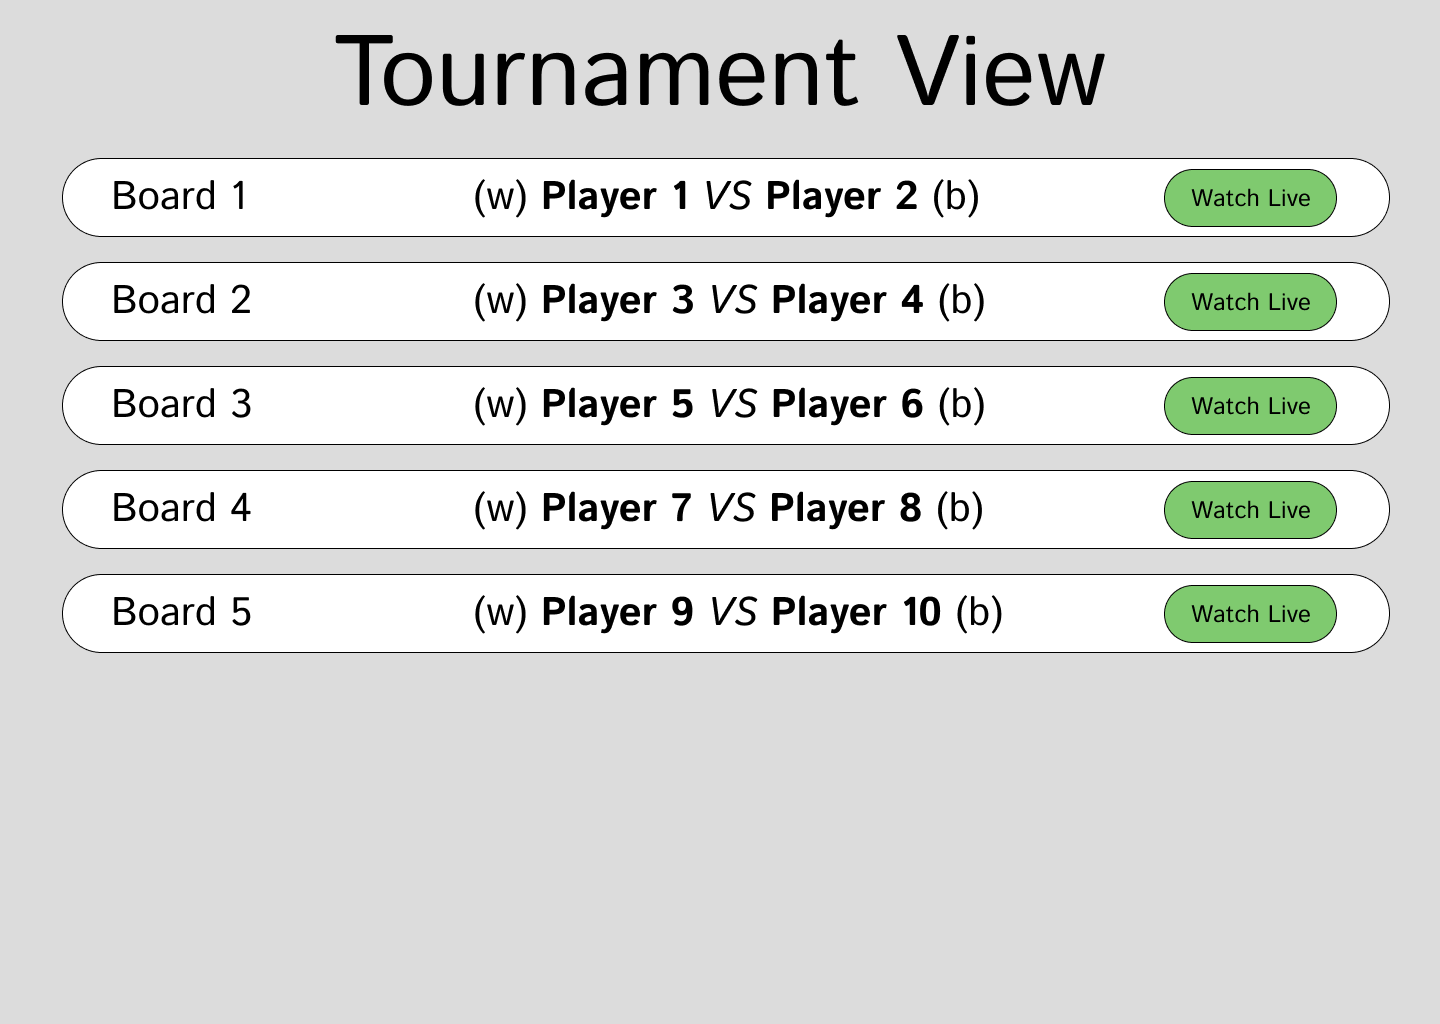
\includegraphics[width=\linewidth]{figures/methods/wireframes/desktop-tournament-view.png}
        \caption{Tournament View}
        \label{fig:desktoop-tournament-view}
    \end{subfigure}
    \hfill
    \begin{subfigure}[h!]{0.45\linewidth}
        \centering
        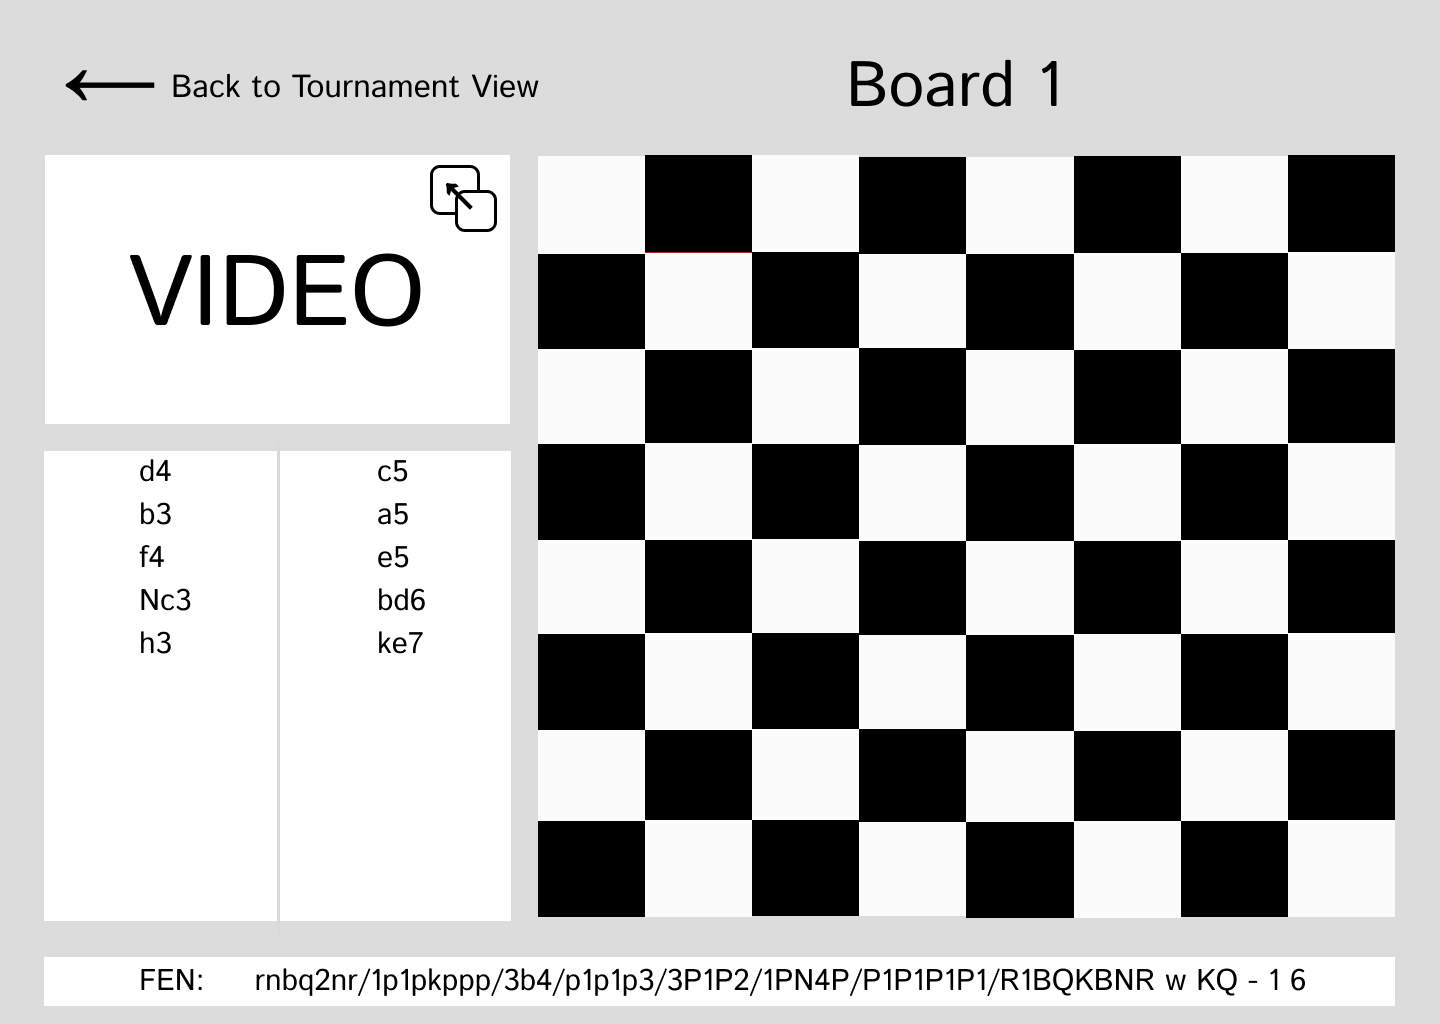
\includegraphics[width=\linewidth]{figures/methods/wireframes/desktop-board-view.png}
        \caption{Board View}
        \label{fig:desktop-board-view}
    \end{subfigure}
    
    \vspace{1em}

    \begin{subfigure}[h!]{0.45\linewidth}
        \centering
        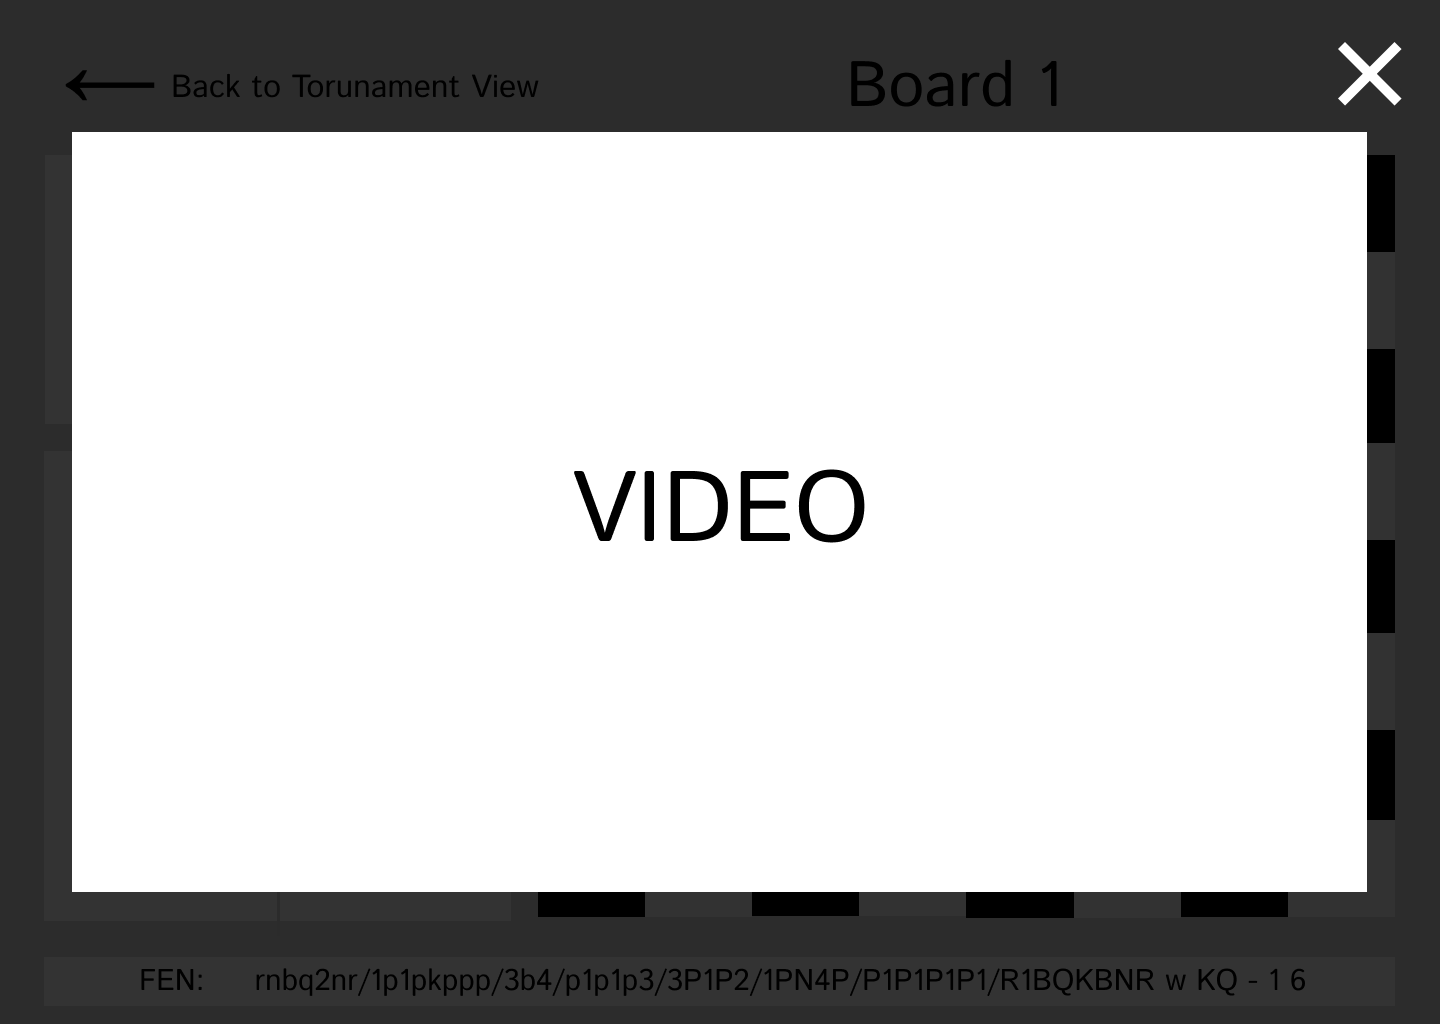
\includegraphics[width=\linewidth]{figures/methods/wireframes/desktop-full-screen-video-view.png}
        \caption{Fullscreen Video Feed}
        \label{fig:desktop-fullscreen-video}
    \end{subfigure}
    
    \caption{Desktop client-side view wireframes}
    \label{fig:desktop-view-group}
\end{figure}

\begin{figure}[h!]
\subsubsection*{Phone View}
    \centering
    \begin{subfigure}[h!]{0.2\linewidth}
        \centering
        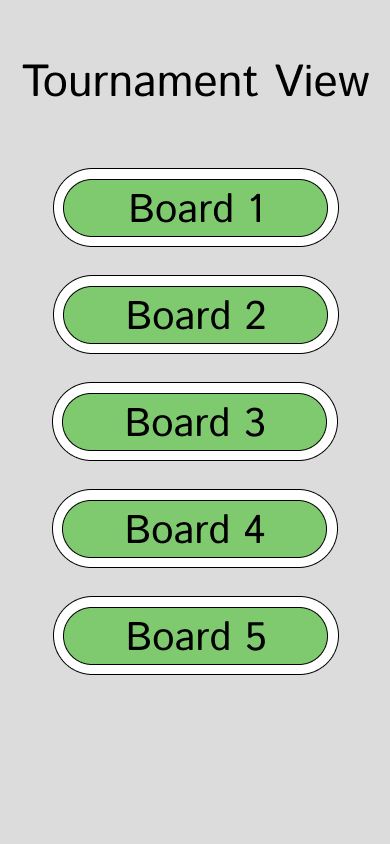
\includegraphics[width=\linewidth]{figures/methods/wireframes/phone-tournament-view.png}
        \caption{Tournament View}
        \label{fig:phone-tournament-view}
    \end{subfigure}
    \hfill
    \begin{subfigure}[h!]{0.2\linewidth}
        \centering
        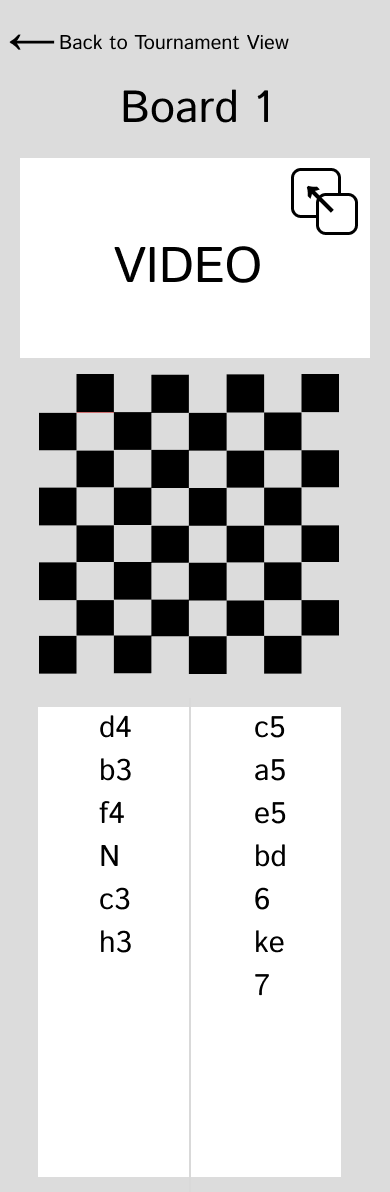
\includegraphics[width=\linewidth]{figures/methods/wireframes/phone-board-view.png}
        \caption{Board View}
        \label{fig:phone-board-view}
    \end{subfigure}
    \hfill
    \begin{subfigure}[h!]{0.2\linewidth}
        \centering
        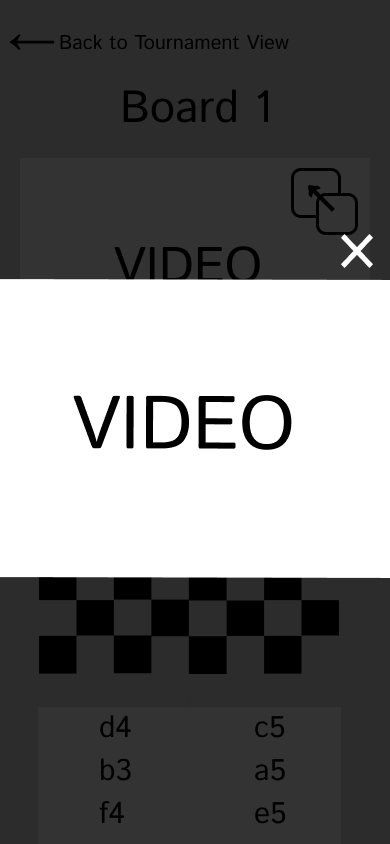
\includegraphics[width=\linewidth]{figures/methods/wireframes/phone-full-screen-video-view-vertical.png}
        \caption{Vertical Fullscreen Video Feed}
        \label{fig:phone-fullscreen-video-vertical}
    \end{subfigure}
    \hfill
    \begin{subfigure}[h!]{0.2\linewidth}
        \centering
        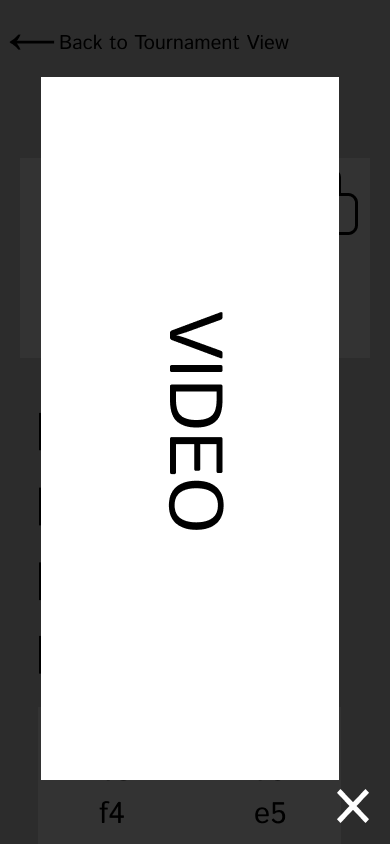
\includegraphics[width=\linewidth]{figures/methods/wireframes/phone-full-screen-video-view-horizontal.png}
        \caption{Horizontal Fullscreen Video Feed}
        \label{fig:phone-fullscreen-video-horizontal}
    \end{subfigure}
    
    \caption{Phone client-side view wireframes}
    \label{fig:phone-view-group}
\end{figure}

\section{Tools and Platforms}
\label{sec:tools-and-platforms}

\subsection{Development Tools}
\label{subsec:development-tools}

\begin{itemize}
    \item \textbf{\gls{vscode}} supports almost every major programming language, making it an ideal all-in-one \gls{ide}.
    \item \textbf{Postman} can test any \gls{api} with pre-configured code snippets: Postman includes a JavaScript-based library of code snippets that enable teams to easily author tests that validate their \gls{api}'s performance, reliability, and behavior.
    \item \textbf{Netron.app} is a visualizer for neural network, deep learning and machine learning models.
    \item \textbf{Git} is a distributed version control system designed to handle everything from small to very large projects with speed and efficiency.
    \item \textbf{\glspl{llm}} are used as an assistance to discuss code quality and structures. Viewed/used as a "sparing" partner.
    \item \textbf{Lighthouse} is an automated tool to help improve quality of web pages.
\end{itemize}.

\subsection{Collaboration and Design Tools}
\label{subsec:collaboration-and-design-tools}

\begin{itemize}
    \item \textbf{GitHub} is used for it's in-house \textit{project} function, creating an Issue Board enabled with easy to use Issues. Also used for code reviewing and code managment.
    \item \textbf{Figma} is a tool used for sketching and creating wireframes.
    \item \textbf{OneDrive} is a platform used for storing files.
    \item \textbf{Overleaf} was used as a report platform, with it's LaTeX support, making it suitable for writing longer reports.
\end{itemize}

\section{Technology Stack}
\label{sec:technology-stack}

\subsection{Backend}
\label{subsec:backend}

For the backend technology, Python is being used.

\subsubsection*{Python Libraries}
\label{subsubsec:python-libraries}

\begin{itemize}
    \item \textbf{chess} is a library for Python, with move generation, move validation, and support for common formats. \cite{python:chess}
    
    \item \textbf{FastAPI} is a modern and fast web framework for building \Glspl{api} with Python. \cite{python:fastapi}
    
    \item \textbf{numpy} is a fundamental package for scientific computing in Python. \cite{python:numpy}
    
    \item \textbf{onnxruntime}, \textbf{onnxruntime-gpu} assists in model serialization and interface with ORT. \cite{python:onnx}
    
    \item \textbf{opencv-python}, \textbf{opencv-contrib-python}, \textbf{opencv-python-headless} is used to solve computer vision problems. \cite{python:opencv}
    
    \item \textbf{requests} allows to send HTTP requests easily. \cite{python:requests}
    
    \item \textbf{scipy} is a fundamental package for algorithms for scientific computing in python. \cite{python:scipy}
    
    \item \textbf{tensorflow}, \textbf{tensorflow-intel} makes it easy to create \gls{ml} models that can run in any environment. \cite{python:tensorflow}
\end{itemize}

\subsection{Frontend}

For the frontend technology, TypeScript is being used. As discussed in \ref{subsec:type-safety}.

\subsubsection*{TypeScript Libraries}

\begin{itemize}
    \item \textbf{Vite} is a fast frontend build tool of web applications. \cite{ts:vite}
    
    \item \textbf{React} builds user interfaces out of individual pieces called components. \cite{ts:react}
    
    \item \textbf{@vitejs/plugin-react-swc} Speeds up the Vite development server. \cite{ts:swc}
    
    \item \textbf{chess.ts} a Typescript chess library for chess move generation/validation, piece placement/movement, and check/checkmate/draw detection \cite{ts:chess}
    
    \item \textbf{react-dom} serves as the entry point to the DOM and server renderers for React. \cite{ts:react-dom}
\end{itemize}